
\documentclass{article}
\usepackage[utf8]{inputenc}
\usepackage{relsize}
\usepackage{amsmath}
\usepackage{geometry}
\usepackage{listings}
\usepackage{tikz}
\usetikzlibrary{automata, positioning, arrows}
\tikzset{node distance=2.5cm, % Minimum distance between two nodes. Change if necessary.
every state/.style={ % Sets the properties for each state
semithick,
fill=gray!10},
initial text={}, % No label on start arrow
double distance=2pt, % Adjust appearance of accept states
every edge/.style={ % Sets the properties for each transition
draw,->,>=stealth', % Makes edges directed with bold arrowheads
auto,semithick}}

\geometry{
 a4paper,
 total={170mm,257mm},
 left=20mm,
 top=20mm,
}

\lstset{
  basicstyle=\itshape,
  xleftmargin=17em,
  literate={->}{$\rightarrow$}{2}
            {e}{$\epsilon$}{1}
}


\title{Homework 4\\[0.2em]\smaller{}CSC 445-01: Theory of Computation}
\author{Matthew Mabrey, Luke Kurlandski}
\date{\today}

\begin{document}

\maketitle

\section*{2.1 (a)-(d)}

\section*{2.4 (b)}
    To generate the language $A = \{w \mid w$ starts and ends with the same symbol$\}$ given $\Sigma = \{0, 1\}$, we create the context-free grammar:
    
\begin{center}
    
    \begin{lstlisting}
    S -> 0X0 | 1X1
    X -> 0X | 1X | e
    \end{lstlisting}
    
\end{center}

\newpage
\section*{2.5 (b)}

The following state diagram represents the pushdown automata that accepts the context-free language $\{w \mid w$ starts and ends with the same symbol$\}$ given $\Sigma = \{0, 1\}$. We begin by pushing the special $\$$ symbol onto the stack to mark the bottom of the stack and then our start symbol $S$. From there we pop $S$ and either push $0X0$ or $1X1$ onto the stack to ensure our string begins and ends with the same symbol. The PDA can then continue adding $0$'s or $1$'s to the stack through the variable $X$ until the special $\$$ is reached. At this point the PDA pops the $\$$ symbol and enters the accept state as our stack is empty and it has successfully created a string that begins and ends with the same symbol.

\begin{center}
    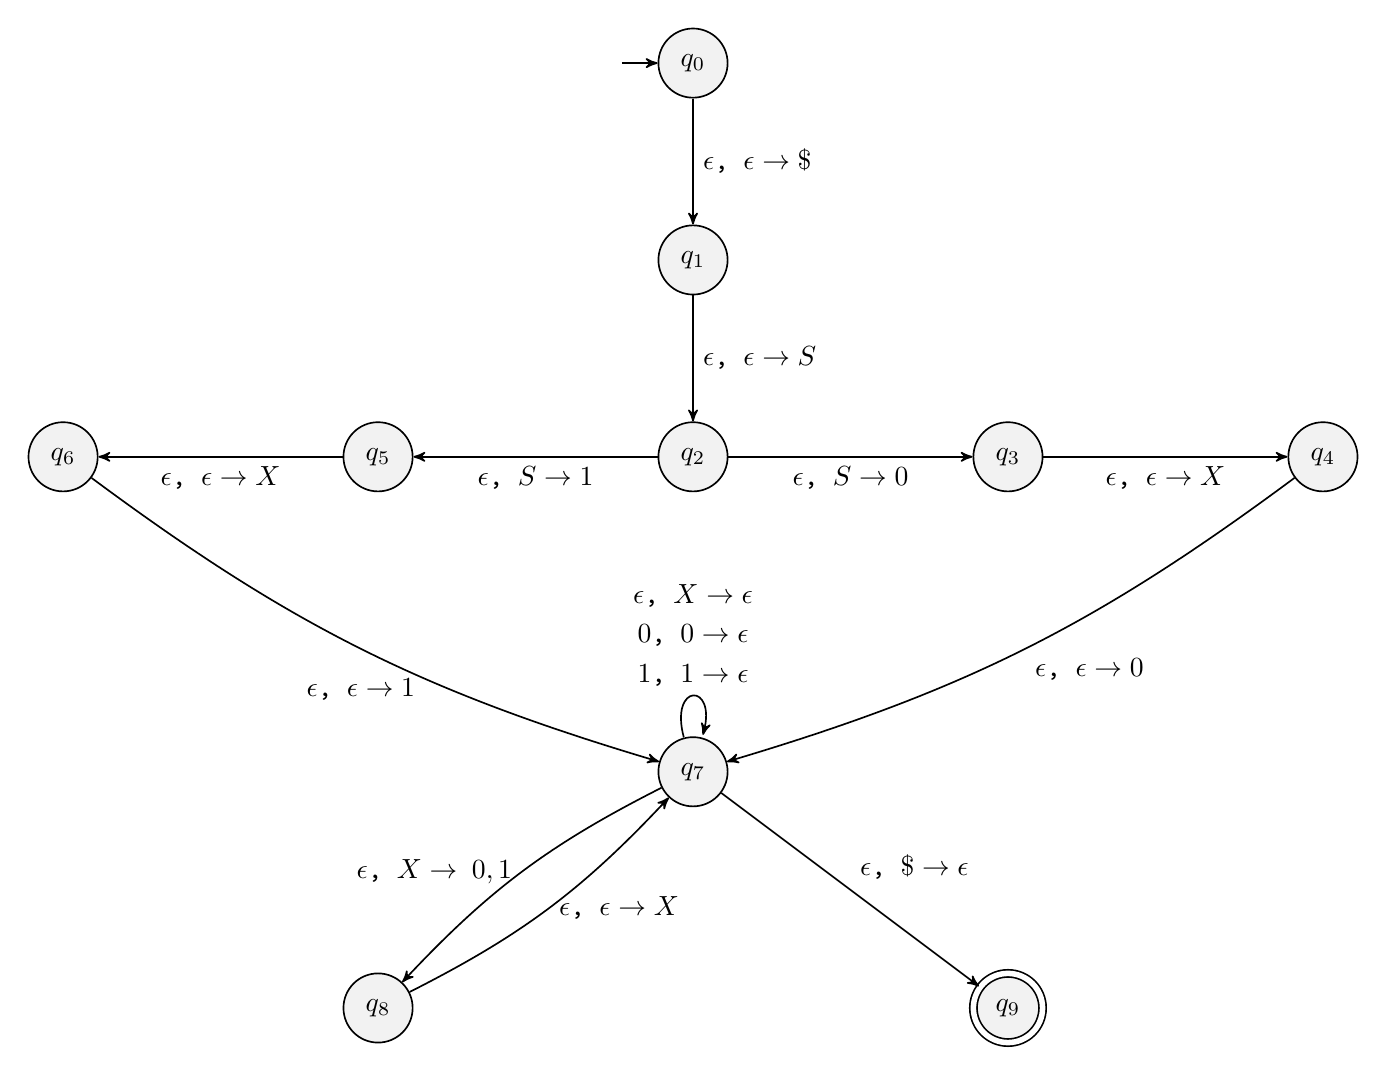
\begin{tikzpicture}
    
    \node[state, initial] (0) {$q_0$};
    \node[state, below of=0] (1) {$q_1$};
    \node[state, below of=1] (2) {$q_2$};
    \node[state, right of=2, xshift=1.5cm] (3) {$q_3$};
    \node[state, right of=3, xshift=1.5cm] (4) {$q_4$};
    \node[state, left of=2, xshift=-1.5cm] (5) {$q_5$};
    \node[state, left of=5, xshift=-1.5cm] (6) {$q_6$};
    \node[state, below of=2, yshift=-1.5cm] (7) {$q_7$};
    \node[state, below of=7, left of=7, xshift=-1.5cm, yshift=-0.5cm] (8) {$q_8$};
    \node[state, below of=7, right of=7, xshift=1.5cm, yshift=-0.5cm, accepting] (9) {$q_9$};
    
    \draw (0) edge node {\tt $\epsilon$, $\epsilon \rightarrow \$$} (1);
    \draw (1) edge node {\tt $\epsilon$, $\epsilon \rightarrow S$} (2);
    \draw (2) edge node[below] {\tt $\epsilon$, $S \rightarrow 0$} (3);
    \draw (3) edge node[below] {\tt $\epsilon$, $\epsilon \rightarrow X$} (4);
    \draw (4) edge[bend left=10] node {\tt $\epsilon$, $\epsilon \rightarrow 0$} (7);
    \draw (2) edge node {\tt $\epsilon$, $S \rightarrow 1$} (5);
    \draw (5) edge node {\tt $\epsilon$, $\epsilon \rightarrow X$} (6);
    \draw (6) edge[bend right=10] node[below, yshift=-0.25cm] {\tt $\epsilon$, $\epsilon \rightarrow 1$} (7);
    \draw (7) edge[loop above, white] node[yshift=1cm, black] {\tt $\epsilon$, $X \rightarrow \epsilon$} (7);
    \draw (7) edge[loop above, white] node[yshift=0.5cm, black] {\tt $0$, $0 \rightarrow \epsilon$} (7);
    \draw (7) edge[loop above] node {\tt $1$, $1 \rightarrow \epsilon$} (7);
    \draw (7) edge[bend right=10] node[above, left] {\tt$\epsilon$, $X \rightarrow$ $0, 1$} (8);
    \draw (8) edge[bend right=10] node[below, right] {\tt$\epsilon$, $\epsilon \rightarrow X$} (7);
    \draw (7) edge node {\tt$\epsilon$, $\$ \rightarrow \epsilon$} (9);
    
    
    
    \end{tikzpicture}
\end{center}
\section*{2.5 (e)}

\newpage
\section*{2.6 (b)}
The CFG that generates the complement for the language $A = \{a^nb^n$ $\mid$ $n \geq 0\}$ is such:
    
\begin{center}
    
    \begin{lstlisting}
    S -> A | bX | aXbXaX
    
    X -> aX | bX | e
    
    A -> aA | e
    
    
    \end{lstlisting}
    
\end{center}

\section*{2.13 (a)}

\end{document}
